%% Copyright Mikko Tuohimaa 2009
%\documentclass[a4paper,12pt]{report}
\documentclass[12pt]{article}

\usepackage[dvips]{graphicx}
\usepackage{url}
%% Matematiikan fontteja, symboleja ja muotoiluja lis��, n�it� tarvitaan usein
\usepackage{amsfonts,amssymb,amsbsy}
%% Taulukon paketti
%\usepackage{multirow}

%% Vaakasuunnan mitat, �L� KOSKE!
\setlength{\hoffset}{-1in}
\setlength{\oddsidemargin}{35mm}
\setlength{\evensidemargin}{20mm}
\setlength{\textwidth}{15cm}
%% Pystysuunnan mitat, �L� KOSKE!
\setlength{\voffset}{-1.5in}
%\setlength{\headsep}{7mm}
%\setlength{\headheight}{1em}
\setlength{\topmargin}{25mm}
\setlength{\textheight}{24cm}
%% Vasensuora-asettelu, joka opinn�ytteess� vaaditaan. �L� KOSKE
\setlength{\parindent}{0pt}
\setlength{\parskip}{1ex}

%% bibtex-tyyli
\bibliographystyle{apalike}

% Title Page
\title{Microfluidic Analyzation, Detection and Testing Methods}
\author{Mikko Tuohimaa}
\date{April 21, 2009}


\begin{document}
\maketitle
\pagenumbering{arabic}
\setcounter{page}{1}
\begin{abstract}
This paper describes various methods of using microfluidic microsystems as 
fast and efficient analyzation
tools for both organic and inorganic compounds. A novel use case in biochemistry
is proposed.
\end{abstract}

\textbf{Keywords:} microfluidics, analyzation, testing, biochemistry

\section{Introduction}
In the area of chemistry and medicine there is a tremendous need for testing methods which are 
cheap, reliable and fast. Conventional testing and analyzation methods usually need a big 
sample and lots of reagents, have long reaction times and thus tend to be expensive. 
Microfluidic devices offer 
a new approach to the task by reducing the volumes needed to the thousandth and thereby 
speeding the process up both by shorter reaction times and also by enabling several different
tests to be run in parallel. Therefore for example all the standard tests for a certain kind of 
disease for a patient in a hospital could be done simultaneously, on a single chip, from a single
sample, providing great value for both the patient and the staff. Scaling effect also enables some sample processing methods not 
available when working with bigger volumes. They are discussed about in 
sections~\ref{section:components} and~\ref{section:detectors}.

Even though microfluidic systems cover a vast field of applications, almost all of them can be
thought of comprising of four basic subsystems: a sampling unit, a processing (microfluidic) 
unit, a detector unit and an electronic controller. In this paper the focus is on processing and
detection while sampling and controlling are problems of distinctly different fields of study.

\section{Basic microfluidic components}\label{section:components}

\subsection{Microchannels}

In microfluidic devices the sample and reagents are handled precisely with micromachined 
channels guiding them. These can be manufactured with a number of technologies, notably 
silicon micromachining and lately polymer molding. Usually the channels are constructed such that 
the machinable substrate is put between layers of glass or silicon, creating sealed tunnels.
The bonds between layers are so strong that actually the substrate's structure itself 
is to cave in before them under pressure.

\subsection{Manipulators}
The basic microfluidic manipulators are pumps and valves, guiding the fluid flow to a desired 
direction. Other components falling into the category are several passive subsystems such as
mixers and separators.

Currently most widely used microvalves and pumps utilize silicon micromachining and a 
piezoelectric film resulting in fast response time and fairly good controllability. Also 
thermopneumatic actuation, where the expansion of heated gas leads to displacement, is 
used, mostly because of the radically lower operating voltage. Usually the structure of a pump 
consists of two valves with the actuator in the middle, sometimes there can also be such 
blocks arranged in a sequence.

In microscale, almost all flow is laminar and thus no mixing happens by turbulence. On the other 
hand, diffusion is an important phenomenon since dimensions are small. Therefore an efficient 
mixer can be constructed like in figure~\ref{fig:mixer}, where the liquids' contact surface 
versus volume ratio and contact time is maximized and grooves are used to affect the flow geometry and therefore the surface shape and area. A simulation on mixing run on a 3D cornered 
mixer is displayed in figure~\ref{fig:mixer_sim}.

Since diffusion is more efficient on 
small particles, an H filter such as in figure~\ref{fig:h_filter} can be used to gradually
extract particles of a specific size. This is very useful because the flow reached is bigger
than when using semipermeable membranes even though the separation result isn't exactly optimal.

\begin{figure}[htcb]
\begin{center}
	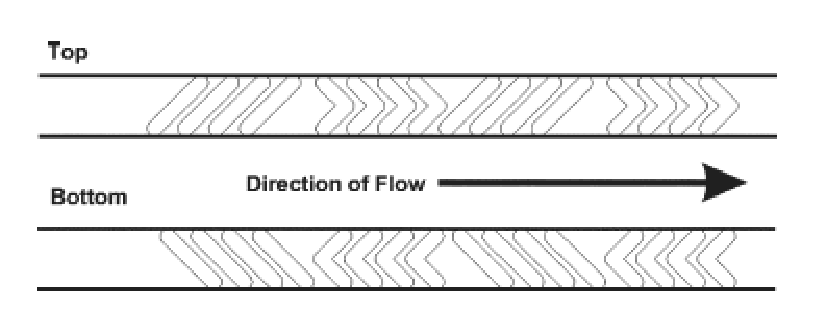
\includegraphics{mixer2.eps}
	\caption{A typical microfluidic mixer \cite{HOWELL_2005}}
	\label{fig:mixer}
\end{center}
\end{figure}

\begin{figure}[htcb]
\begin{center}
	
\includegraphics{mixer.eps}
	\caption{A simulation run on a fictitious microfluidic mixer~\cite{TECPLOT}}
	\label{fig:mixer_sim}
\end{center}
\end{figure}

\begin{figure}[htcb]
\begin{center}
 	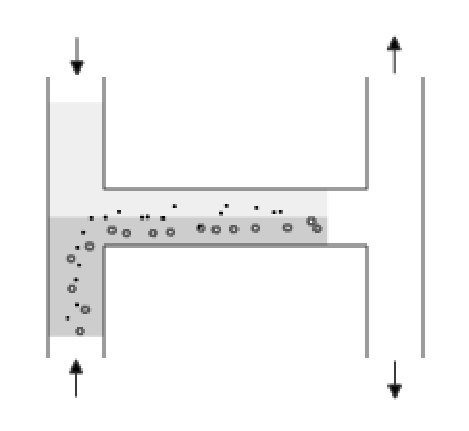
\includegraphics{h_filter.eps}
	\includegraphics{h_filter2.eps}
	\caption{The basic operating principle of an H filter: small particles diffuse more efficiently than big ones}
	\label{fig:h_filter}
\end{center}
\end{figure}



\section{Detectors}\label{section:detectors}

\subsection{Optoelectronic detection methods}
Optics can be used to detect characteristics of the sample in various ways. Some reactions
change the sample's light absorption properties, specifically its absorption spectrum~\cite{SUGINO_2009},
which can be detected with an active sensor, some on the other hand rely on (bio)luminescence
and fluorescence, ie. when activated and stimulated the reagent emits photons which can be detected~\cite{KAMEI_2008}.

The detection itself is done with photodiodes with sufficient filters and possible lens systems.
The challenging
part is to develop such a testing method that the optical response is detectable, accurate and
gives few false results. Often these methods include using a (bio)receptor which activates the
luminous substance when in contact with the particle to be detected. For example in DNA 
microarrays each cell of the array contains picomoles of a specific oligonucleotide which
corresponds to a specific DNA sequence (usually a gene), and the result is somewhat like in
figure~\ref{fig:dna_microarray}. Other methods include detecting the presence of transition 
element ions based on colorimetry since each element absorbs light at different wavelengths. 
Transition elements can also be used to form larger molecules with the substances in the sample, 
thus resulting in a different color and the detection of eg. oxygen.

\begin{figure}[htcb]
\begin{center}
	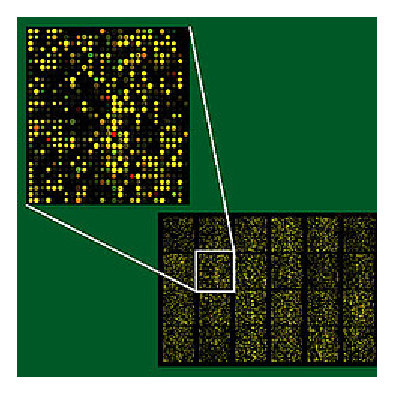
\includegraphics{dna_microarray.eps}
	\caption{Sample output of a DNA microarray}
	\label{fig:dna_microarray}
\end{center}
\end{figure}


A more high-end approach is to use an evanescent wave technique where the detector 
comprises of a 
microscopic gold layer on a high refractive index glass surface. The gold layer can absorb 
light at a specific angle and wavelength, producing electron waves. This is highly dependent
on the surface of the gold so that binding of target molecules on the surface's receptors 
results in a measurable change of the surface's reflective properties. This can be measured
accurately.~\cite{ZOUROB_2007}

\subsection{Electrochemical methods}
Most electrochemical detectors catalyse and detect reactions producing or consuming 
electrons, eg. acid neutralization. The amount of ions produced or consumed by the 
reaction is detected with an ISFET (ion-sensitive field effect transistor)~\cite{yotter_2004} 
or by performing the reaction on an electrode and measuring the 
resulting current amperometrically~\cite{yotter_2004}. Since reaction speed and with
it the signal strength is mostly
dependent on the electrode area, various approaches have been developed to maximize
its area-to-volume ratio which also is the main affector of the sensor's signal-to-noise
ratio.

Electrochemical sensors are mostly used to detect pH and, especially in biochemical detection, levels of oxygen, carbon dioxide, glucose,
adenosine triphosphate, hydrogen, methane, nitrate, sulphate and some other substances
dissolved in the sample~\cite{yotter_2004}, but also biological macromolecules such as specific
genes can be detected~\cite{wu_2008}. The target substance is selected with electrode material, also 
sometimes additional enzymes and semipermeable membranes are used to restrict the reaction
to a single target substance.

The downside of the method is that the substance detected is consumed in the reaction 
which can even be fatal when analyzing living cells. That's why sometimes the sensor is
equipped with a counter electrode which aims to catalyse the reverse reaction thus 
maintaining equilibrium.

\subsection{Capillary electrophoresis (CE)}
Capillary electrophoresis can be used to separate ionic species by their (surface) charge 
and frictional forces. Introduced in the 1960s, CE was designed to separate species based 
on their size to charge ratio in the interior of a small capillary filled with an electrolyte.
The instrumentation needed is relatively simple:
the capillary is dipped to the sample vial, then placed in the source vial. Both vials
contain an electrolyte, such as an aqueous buffer solution. The migration of the analytes is
initiated by a strong electric field applied between source and destination vials, resulting 
in all ions (positive \textit{and} negative) to be pulled through the capillary due to
electroosmotic flow. The analytes separate as they migrate due to their electrophoretic mobility
and are detected near the outlet end of the capillary. The data collected is shown as an 
electropherogram, which reports detector response as a function of time: separated chemical 
compounds appear as peaks with different retention times.~\cite{SKOOG_2006}

\subsection{Other methods}
Detection methods other than those described above are rather uncommon but still interesting.
Eg. a change in standing wave resonance frequency can be used to determine the amount of 
particles attached to a piezoelectrically vibrated beam coated with receptors. The accuracy 
of this method can be greatly increased using surface wave modes since the weight ratio of 
vibrating mass to the additional mass decreases dramatically.~\cite{GRATE_2000}

\section{Common use cases}
Microfluidics is a rapidly developing science and new applications are developed continuously.
In the following sections a few common commercial cases are introduced.

\subsection{DNA Microarrays}
A DNA microarray is a multiplex technology used mainly in medicine and microbiology. It consists
of an array of DNA receptors, usually oligonucleotides, each of which corresponds to a distinct
DNA sequence. The receptors can be labelled with a fluorescent or a chemiluminescent agent enabling
visual detection of a match.

DNA microarrays have had a great impact on genetic research after first being published in 
1995~\cite{SCHENA_1995}, being a fast, reliable and rather cheap method of DNA sequencing.
Especially exploratory genetic research has benefitted of the advances on this area since 
microarrays enable not only the study of a genome but also the expression of genes as a function 
of time: for example one can extract mRNA from a cell and again after some time, within the same cell cycle 
or maybe after several
mitoses. Then, the cDNA reverse transcripted from the mRNA samples can be labeled with 
different agents (say green and red fluorescents) and used as a hybrid sample on a DNA microarray.
Then it's possible to measure the ratio of expression of each gene by observing the intensities of
different labels (figure \ref{fig:expression}). Such research was more or less impossible before
microarrays were introduced because of the time and big samples the previous methods needed to 
function.

\begin{figure}
 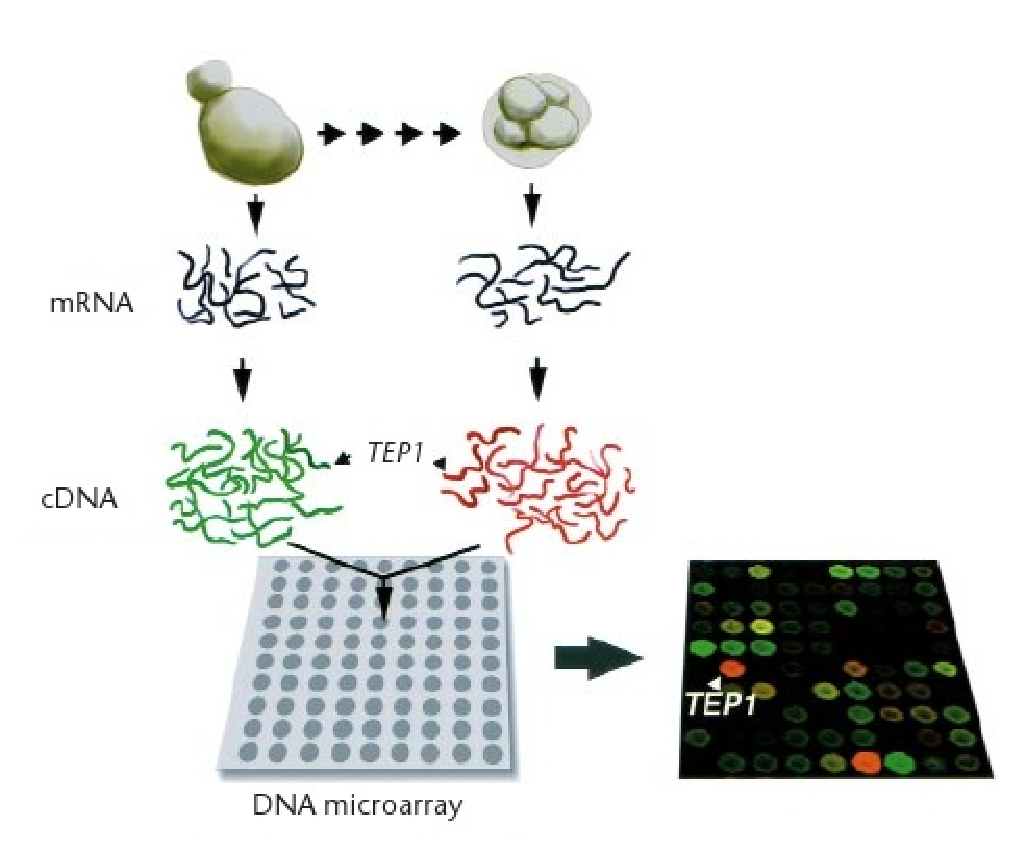
\includegraphics[scale=0.75]{gene_expression.eps}
 \caption{An example of comparative analysis of gene expression \cite{BROWN_1999}}
 \label{fig:expression}
\end{figure}

DNA microarrays, as all the other types of microarrays, can be assembled on a glass, polymer or silicon 
surface. Depending on the desired features and cost of the array, surface micromachining can be used
to maximize the chip's surface-to-volume ratio thus enhancing the signal: eg. Chen, et al. have developed
a porous matrix based microfluidic chip for DNA extraction that has a surface area to volume ratio of
$300 m^2/cm^3$. The DNA receptors, \textit{probes}, are then assembled as a matrix on the surface
with one of a number of technologies including printing with fine-pointed pins,
photolithography using pre-made masks, photolithography using dynamic micromirror devices, ink-jet 
printing~\cite{LAUSTED_2004}, and electrochemistry on microelectrode arrays. The number of probes can
be anything from a dozen to several million depending on the application~\cite{KIM_2005}.

\subsection{Pathogen detection}
During the last ten years, several different methods have been developed to detect the presence of 
both viruses and bacteria. This can be accomplished by detecting the microbes directly or by
detecting their metabolic products. The test can be done on specific virii and bacteria or more
generically, just identifying the type of pathogen present.

Portia Briones et al. developed a microfluidic device for detection of human cytomegalovirus (CMV)~\cite{BRIONES_2006}.
Their method is to amplify the CMV DNA via PCR (Polymerase Chain Reaction) and then detect it using
complementary PNA (peptide nucleic acid) probe in a microchannel: both reagents are injected to the
same channel, resulting in a laminar flow in the straight part of the channel. The hybridization between the target and the probe 
occurs at the interface of the laminar flow. Secondary laminar flow, on the other hand, is formed at the
curving part of the microchannel allowing separation of DNA hybrids. The hybrids are detected by laser induced
fluorescence microscopy near the end of the channel (figure \ref{fig:cmv}). The method proposed has several
advantages, such as fast reaction time, ability to detect even the smallest amounts of viral DNA thanks to
PCR and low cost compared to traditional methods.

\begin{figure}
 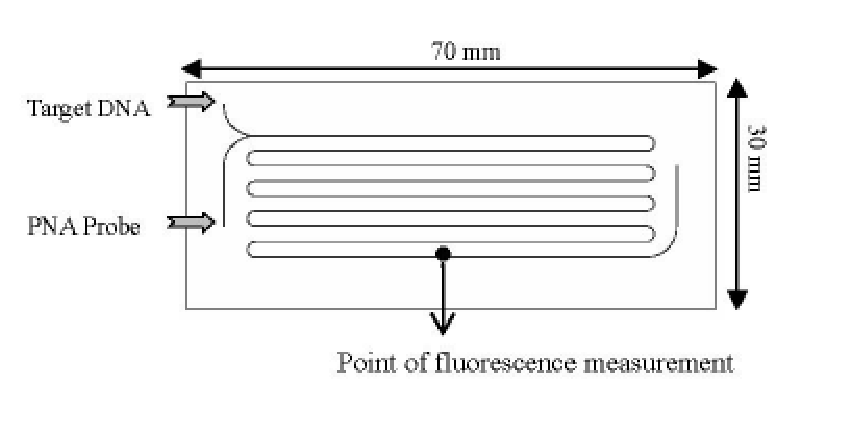
\includegraphics{cmv.eps}
 \caption{A microfluidic configuration for detecting human cytomegalovirus~\cite{BRIONES_2006}. The curves affect the 
laminar flow present in the channel, resulting in desirable dynamics.}
 \label{fig:cmv}
\end{figure}

Huang et al. have developed a fully-integrated microfluidic chip for RNA virus detection~\cite{HUANG_2005}. The sample is 
amplified using reverse transcription polymerase chain reaction (RT-PCR), the resulting RNA/DNA strains
are then separated by capillary electrophoresis (CE) and detected using buried optical fibres. The
method used allows detection of any RNA virus, depending on the selectivity of RT-PCR.

Mai et al. have come up with a MEMS electrochemical biosensor to detect pathogenic bacteria in urine. Using custom-designed
DNA oligonucleotide probes specific for bacterial RNA, species-specific detection was achieved within
45 minutes. In their solution, though, the sample preparation was still a labour-intensive 7 to 10
step process. Their aim is to develop an integrated microfluidic chip capable of the preparation 
process and compatible with the existing biosensor, resulting in a lab-on-a-chip for rapid
bacterial pathogen detection.~\cite{MAI_2007}

\subsection{Glucose level sensing}

Glucose sensing is extremely important commercially,
since diabetics need to keep control of their blood glucose to
prevent either hypoglycaemia or hyperglycaemia. The early
sensors tested for ketones in urine, which are indicative of
raised blood glucose levels. However the delay in
metabolism of glucose to ketone metabolites prevented close
monitoring of blood glucose. The big advance in direct
measurement of blood glucose came when the enzyme glucose
oxidase (GOD) became widely available. Glucose
oxidase oxidises glucose to gluconic acid, liberating hydrogen
peroxide, which can then be electrochemically and optically
detected.~\cite{YU_2008}

Huang, et al. have developed an integrated, hand-held microfluidic device which measures blood glucose level
real-time and automatically injects the proper amount of insuline if needed.~\cite{HUANG_2006} Compared to separate detection 
and insuline injection systems, the solution offers the benefit of simplicity and precise dosing of insuline.
The system is fabricated by using microfluidic techniques comprising of glucose sensing electrodes, a flow sensor and
polydimethylsiloxane (PDMS)-based microfluidic structures such as micropumps, microvalves and microchannels. Commercially 
available needles are incorporated for continuous glucose monitoring and long-term insulin injection.

\section{Use proposition: Lab-on-a-chips for home use}

When sick with a common cold, people are often facing a tough choice: to go to the doctor or not. With current home
appliances it's rather difficult to determine if eg. antibiotics are needed. A solution for this
could be a cheap, simple lab-on-a-chip which would determine a few key points about the disease,
primarily if it's viral or bacterial. If viral, there's no point in going to get checked 
since even the most modern medicine can't do much more than suggest a lot of rest and hot beverages, while
bacterial infections can and often should be treated with antibiotics. Considering the amount of doctors' 
time spent on insignificant visits, a self-applied preliminary test could offer huge savings on medical 
expenses and be convenient for the patient.

The key to this application's commercial success is a low price tag and a very simple user interface.
The former can be obtained by the fact that the analyzer needs to do nothing more than determine if
the patient should consult a doctor or not; the measurements can be crude and there doesn't need to be that 
many of them. The latter on the other hand depends on whether the test can be done on saliva or other
bodily fluids or is a blood sample necessary.

\bibliography{seminar}

\end{document}          
